\chapter{Implementation} \label{chap:Implementation}
This chapter presents the implementation details of the CRI extension. In the first section, we present two alternative implementations of the CRI extension. The second section describes the significant data structures used by the extension. The communication in between different components of the extension is explained in the third section. The fourth section presents the developed query language and its usage. The last section describes the graphical user interface provided by the extension.

\section{CRI - Implementation Alternatives }
In this section, we present two possible implementations of CRI extension. To determine the best possible alternative is yet to discover by looking into the pros and cons of both alternatives and is mentioned as one of the possible future work. We tried our hands at both alternatives, but for the final version, we focused on the first alternative. So except this section, everything presented in this thesis is based on the first alternative. 


\subsection{Alternative - 1}


As described in section~\ref{subsec:Extending_Chrome_DevTools}, in Chrome DevTools extesnsion, page script and content script runs in two different execution contexts, and both have access to same DOM.
Figure~\ref{fig:system_implementation_detail_1} depicts component level details of the first alternative, where the user has an application with reactive
code to debug or analyse. Before execution takes place, the application code is intercepted by DevTools extension and the manipulated code is run in the browser which provides the same output as the original code.
All components residing within the big dotted round cornered box are run as a content script. \textbf{Interceptor} module is responsible for preventing JavaScript code in the target application from executing in the browser. For this purpose, we created a script that runs as a content script at document start. It uses \textbf{window.stop} to halt the normal loading of the web page to the browser. 
Then, we make a XHR(XMLHttpRequest) request to get the content of the target document. Replace the \textbf{type} attribute of all script tags with some custom string and write it to the document, this will stop the browser to execute that script. After that sequentially loads the JavaScript files and instruments them if required and injects them into the web page as a content script.
After instrumentation, when manipulated code runs in the browser then it invokes the Jalangi API on
different events like whenever any value is written to JavaScript variable.
Instrumentor receives JavaScript code from the interceptor module and performs instrumentation on a given JavaScript code with Jalangi library. Instrumentor returns instrumented code to the interceptor module. 


\begin{figure}[!h]
	\centering
	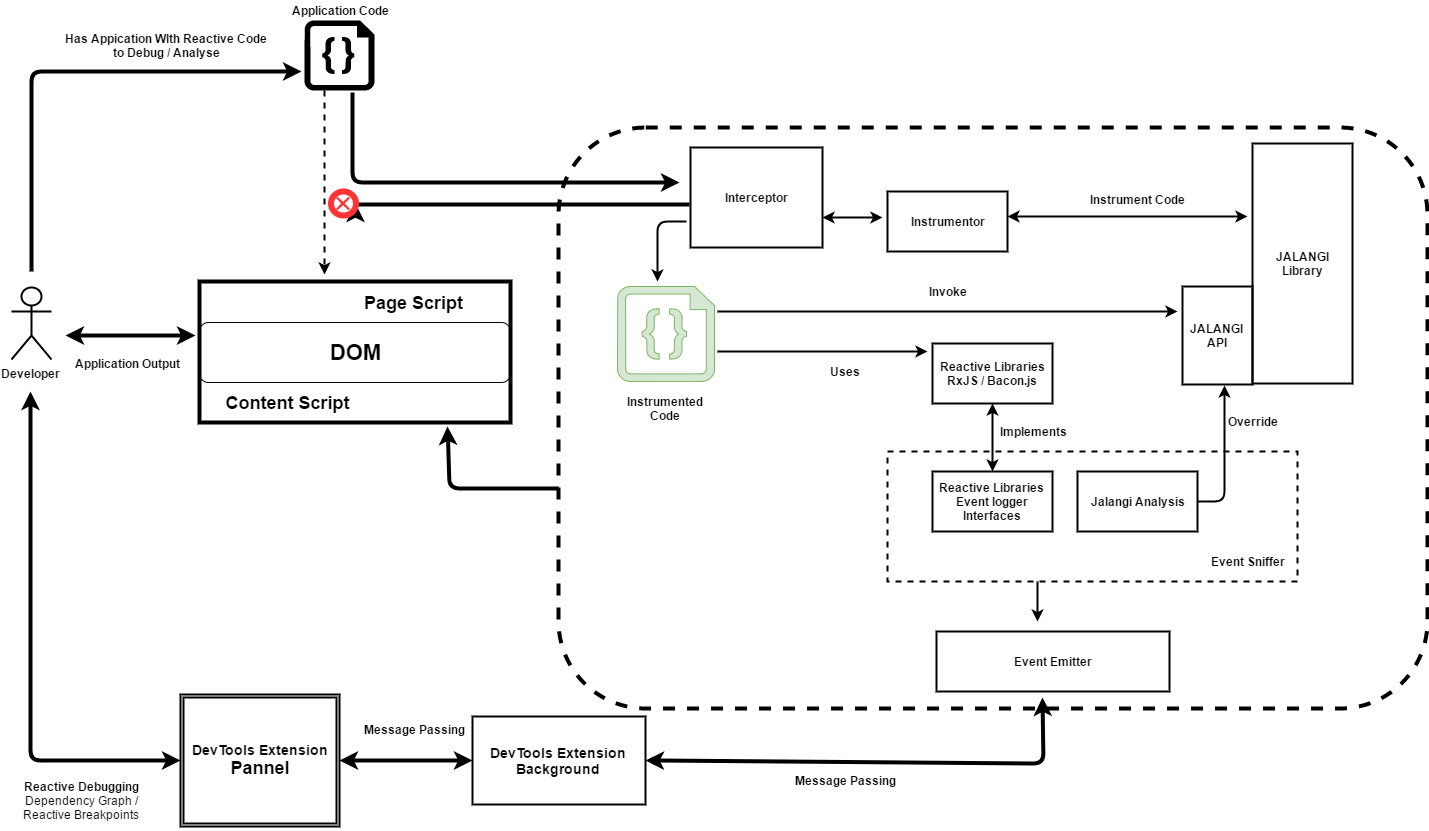
\includegraphics[width=\textwidth,height=\textheight,keepaspectratio]{gfx/SystemFlowDiagramDesign1.png}
	\caption{System Components Detail - Alternative 1}
	\label{fig:system_implementation_detail_1}
\end{figure}


\textbf{Event sniffer} comprises of two sub-components,
the first one contains the reactive library specific implementation to log all internal activities such as the creation of observable, and values emitted to subscribers.
The second sub-component of Event sniffer is Jalangi Analysis that overrides some methods of Jalangi API, which make it possible to map the reactive streams to the JavaScript variable name.
Event Emitter is also part of the content script, it receives events information from event sniffer, it changes them to defined message structure and passes this as a message to extension\textquotesingle s background page.
The communication in between content script, background page and extension panel is done with message passing  \footnote{\url{https://developer.chrome.com/extensions/messaging} , last accessed 24-05-2017}. 
Extension\textquotesingle s background page receives messages of a defined pattern from the event emitter and passes them to extension panel.
Similarly, background page also receives messages from extension panel and forwards them to content script.
Extension\textquotesingle s panel receives events information as a message from background page, parse those messages and responds according to the type of the message.
The message can be of type \textbf{saveNode} or \textbf{saveEdge}. If the message type is \textbf{saveNode} then we check whether it is an update to an existing node or it is a new node.
On receiving a message from the background page, extension panel update the dependency graph and save the graph state in the browser storage. Whenever the new state of dependency graph is saved to the browser storage, the step slider is also updated.
Finally, the developer sees the updated dependency graph, to which he can interact with by setting reactive break points or navigating through the history of the dependency graph. 







\subsection{Alternative - 2}  \label{subsec:Alternative_2}





\begin{figure}[!h]
	\centering
	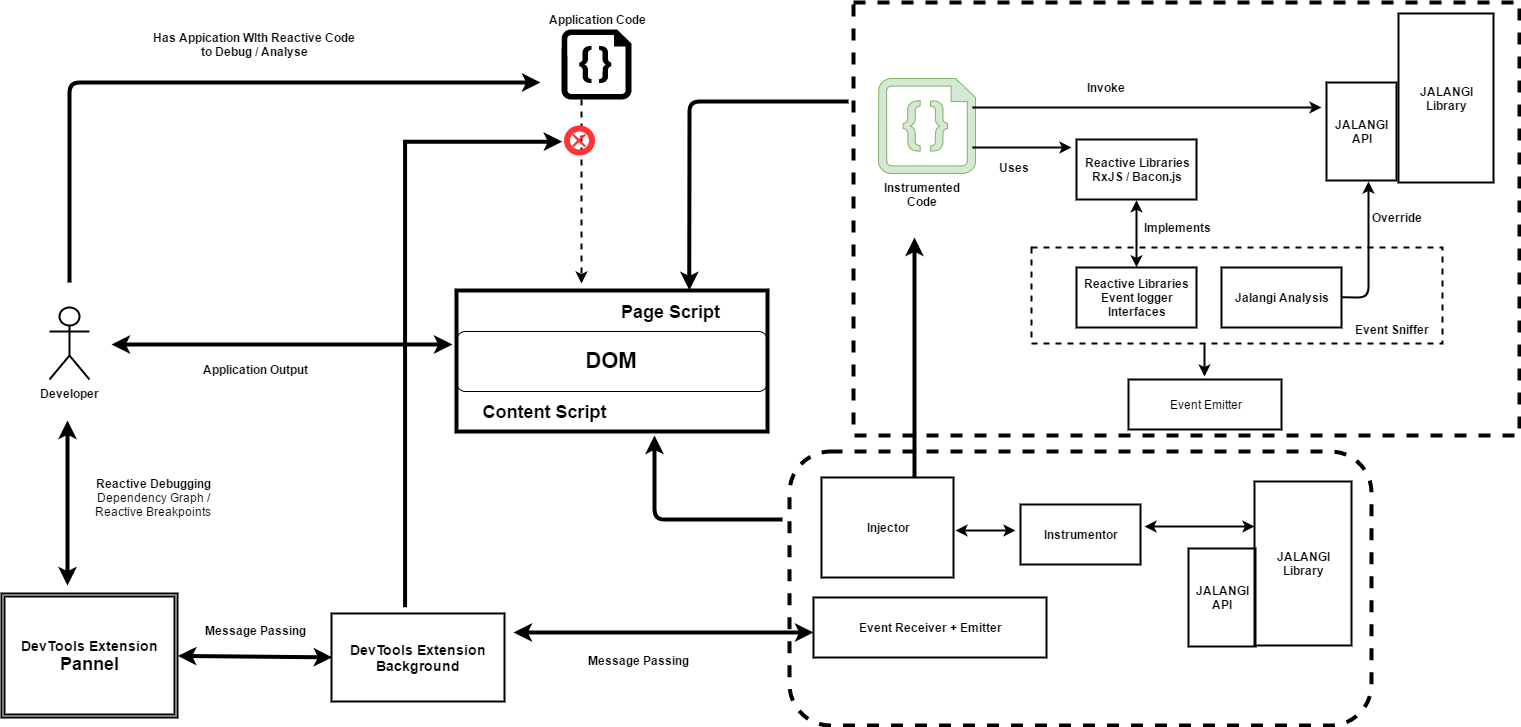
\includegraphics[width=\textwidth,height=\textheight,keepaspectratio]{gfx/SystemFlowDiagramDesign2.png}
	\caption{System Components Detail - Alternative 2}
	\label{fig:system_implementation_detail_2}
\end{figure}

Figure~\ref{fig:system_implementation_detail_2} presents the implementation details of the second approach. Most of the modules are common to the first option.
With this approach, instead of preventing the whole page from loading to the browser, we use \textbf{chrome.webRequest}\footnote{\url{https://developer.chrome.com/extensions/webRequest} , last accessed 25-05-2017} API in background page of the extension to only intercept the HTTP request to specific files that are defined in the field of the scoping feature.
Injector script is run as a content script by extension at the end of the document loading; it is responsible for getting target JavaScript files with XHR request and instrumenting it with Jalangi. 
All modules within the dotted square box are injected by injector script into the target web page as page scripts. Event sniffer works similarly as in the first approach.
Event emitter from the page script passes messages to \textbf{Event receiver + emitter} using \textbf{Window.postMessage()}\footnote{\url{https://developer.mozilla.org/en-US/docs/Web/API/Window/postMessage} , last accessed 25-05-2017}, which is then received in the content script by \textbf{Event receiver + emitter} .
From here onwards everything works as described in the first approach.
The noticeable differences in this method are as follows: 
1) instrumented code, and event sniffer modules run in page script context.
2) Intercepting of target JavaScript code is being done from background script of extension.




\section{Significant Data Structures}

There are two important data structures defined in CRI. The first one is used while sending a message from content script to the panel and the other is used while saving the history of dependency graph into Chrome storage. Listing~\ref{lst:imp_sig_data_structs} shows those significant data structures.

In CRI, the communication between content script (event emitter) and the panel has a defined data structure. 
The message object has two attributes named as \textbf{content} and \textbf{action}.
The \textbf{action} attributes define which type of event has occurred, and the \textbf{content} attribute contains detailed information about that message. Two important values of action attribute are \textbf{saveNode} and \textbf{saveEdge}.\\
In the case of \textbf{saveNode}, the \textbf{content} attribute contains \textbf{node} object and \textbf{node} object contains the following properties:\\
\begin{itemize}
\item \textbf{nodeId}: defines the unique id of the node.
\item \textbf{nodeType}: specifies the type of reactive variable, it can be observable, eventStream or property. Different reactive libraries have their own implementations for time-changing variables.
\item \textbf{nodeMethod}: determines the method name which results in this stream.
\item \textbf{nodeRef}: contains the JavaScript variable name, identified by jalangi. It can be empty in the case of intermediate streams; those are not directly assigned to a variable.
\item \textbf{nodeValue}: contains the current value of this reactive variable as a string.
\item \textbf{sourceCodeLine}: holds the line number from the source code, where this reactive variable is defined.
\end{itemize}
In the case when \textbf{action} attribute of the message is set to \textbf{saveEdge}, the \textbf{content} attribute contains edge object and \textbf{edge} object is defined by the following properties:\\
\begin{itemize}
\item \textbf{edgeStart}: The node id of the parent reactive variable, on which another reactive variable depends.
\item \textbf{edgeEnd}: The node id of the child reactive variable, which results in the application of some operator on parent reactive variable.
\item \textbf{edgeLabel}: The name of the operator which causes this dependency.
\end{itemize}

\begin{lstlisting}[language=JavaScript, caption=Significant Data Structures used by CRI, label={lst:imp_sig_data_structs}]
// Message object in case of dependency creation
{
	content: {
		"edgeStart": '',
		"edgeEnd": '',
		"edgeLabel": ''
	},
	action: "saveEdge",
	destination: "panel"
}

// Message object in case of new reactive stream defined / existing stream gets a new value
{
	content: {
		'nodeId': '',
		'nodeType': '',
		'nodeMethod': '',
		'nodeRef': '',
		'nodeValue': '',
		'sourceCodeLine': ''
	},
	action: "saveNode",
	destination: "panel"
}

// Data Structure for history of dependency graph
{
	"stageId": '',
	"stageEvent": '',
	"stageCurrentNode": '',
	"stageCurrentEdgeStart": '',
	"stageCurrentEdgeEnd": '',
	"stageData": {
		"nodes": [],
		"edges": []
	}
}
\end{lstlisting}

History of dependency graph is saved to chrome storage as an array of \textbf{stage} objects, and \textbf{stage} object comprises of the following properties. Each stage represents a single step of the history of the dependency graph.\\
\begin{itemize}
\item \textbf{stageId}: represents the id of the stage/step for the history of the dependency graph.
\item \textbf{stageEvent}: represents the event that causes this stage. (saveEdge, newNode, updateNode)
\item \textbf{stageCurrentNode}: represents the id of the current node. It is used to highlight a node in the dependency graph.
\item \textbf{stageCurrentEdgeStart}: If current stageEvent is saveEdge then this property contains the parent node id.
\item \textbf{stageCurrentEdgeEnd}: If current stageEvent is saveEdge then this property contains the child node id.
\item \textbf{stageData}: is an object that contains an array of all nodes and edges objects.
\end{itemize}

\section{Communication between Extension Components}

Since the content scripts run in the context of a web page and not the extension, they often need some way of communicating with the rest of the extension. In our case of CRI implementation, event sniffer script run as a content script. It has to forward the information about logged events from reactive libraries to the panel, which further reacts to those messages by updating dependency graph in the panel GUI and saving this information to browser storage for later access. Communication between extension components works by using message passing.
Two possible ways to communicate between extension components are simple one-time requests and long-lived connections\footnote{\url{https://developer.chrome.com/extensions/messaging} , last accessed 26-05-2017}.
We use long-lived connections because event sniffer would send messages continuously. Extension\textquotesingle s panel creates a channel to background script with the name \textbf{reactive-debugger} and adds listeners to receive messages from the background script.
Listing~\ref{lst:imp_comm_panel_code} shows the relevant code that panel script uses to create a connection with background script.


\begin{lstlisting}[language=JavaScript, caption=Panel Script to Communicate with Background, label={lst:imp_comm_panel_code}]
//Create a port with background page for continuous communication
var port = chrome.extension.connect({
	name: "reactive-debugger" //Given a Name
});
// Listen to messages from the background page
port.onMessage.addListener(function (message) {
	// Here we get message from background,
	// that gives us information about events like,
	// New reative variable is defined / Dependency established / New value of reactive stream
	
});
\end{lstlisting}

Listing~\ref{lst:imp_comm_background_code} shows the relevant code for background script to communicate with content scripts and panel script.
To handle incoming connections in background script, we set up an \textbf{extension.onConnect} event listener. When \textbf{extension.connect} is called from the panel script, \textbf{extension.onConnect} event is fired along with \textbf{runtime.port} object that we can use to send and receive messages through that connection. 
The \textbf{Event Emitter} module of CRI which also runs as content script send messages to background script by using \textbf{chrome.extension.sendMessage}, which is received by background script and forwarded to panel script.

As in the second alternative~\ref{subsec:Alternative_2}, the event emitter is injected into the web page context instead of running as content script so in this case the event emitter passes messages that it receives from event sniffer to the content script by using \textbf{window.postMessage} , which is received in content script \textbf{Event Reciever + Emitter} module.
Beside direct communication between extension components by message passing, there is an indirect communication which is being done by \textbf{chrome.storage} API already explained in section~\ref{subsec:Data_Storage_and_mgmt}.

\begin{lstlisting}[language=JavaScript, caption=Background Script to Communicate with Panel and Content Scripts, label={lst:imp_comm_background_code}]
chrome.extension.onConnect.addListener(function(port) {

	// Listens to all incoming messages
	// Message can be from content script or from panel
	chrome.extension.onMessage.addListener(extensionListener);
	
	// function to identify message source and forward its destination
	var extensionListener = function(message, sender, sendResponse) {
		// identify destination of message and forward it
		if (message.destination == "panel") {
			// message from content script so send it to panel
			port.postMessage(message);
		} else {
			if (message.tabId && message.content) {
				// message from panel and send to content script
				chrome.tabs.sendMessage(message.tabId, message, sendResponse);
			} else {
				// message from content script and send to panel script
				port.postMessage(message);
			}
		}
		sendResponse(message);
	}

	// Remove message listner when we close DevTools window
	port.onDisconnect.addListener(function(port) {
		chrome.extension.onMessage.removeListener(extensionListener);
	});
});
\end{lstlisting}


%\section{Dependency Graph Visualisation}
\section{The Query Language}  \label{sec:The Query Language}
Two important features of the CRI extension are based on query language.\\ 
A) Querying the dependency graph history after the execution of the application.\\ 
B) Setting reactive-programming specific breakpoints.\\ 

Let\textquotesingle s take a deeper look into the implementation of these two features.

The single commands are listed and explained in Table~\ref{table:imp_query_lang_for_history}.
The commands for feature \textbf{A} is based on nodeName\textquotesingle s and for feature \textbf{B} commands are based on nodeId\textquotesingle s.
In the first feature, extension gets the query when the user submits the query and it parses the submitted query with regular expressions. By applying regular expression we identify the query and its parameters. After identifying the query and its parameters, we apply the search operation to the data of dependency graph.
For the second feature, panel script stores the submitted queries in chrome storage and accesses it from the content script. The content script parses then those queries to apply breakpoint on the relevant place of the code.


\begin{table}[h!]
	\small
	\begin{center}
		\begin{tabular}{|l|l|p{3cm}|}
			\hline
			Command & Parameters & Description \\ \hline
				nodeCreated[nodeName] & nodeName: name of the node &  specific node is created \\ \hline
				nodeUpdated[nodeName] & nodeName:  name of the node &  specific node is updated, e:g node gets a new value \\ \hline
				evaluationYielded[nodeName][value] & \vtop{\hbox{\strut nodeName:  name of the node}\hbox{\strut value: a String}}   &  evaluation of specific node yields specific value \\ \hline
				dependencyCreated[nodeName1][nodeName2] &  \vtop{\hbox{\strut nodeName1:   name of the parent node}\hbox{\strut nodeName2:  name of the child node}} &  dependency between two specific nodes is created \\ \hline
			%	evaluationException[nodeName]  & nodeName: a name of a node &  evaluation of specific node throws an exception \\ \hline
		\end{tabular}
	\end{center}
	\caption{Commands of the Query Language}
	\label{table:imp_query_lang_for_history}
\end{table}




\section{Graphical User Interface}
\label{Graphical_User_Interface}
The graphical user interface of the debugger is Chrome DevTools panel view which can be opened just like any other panel in DevTools. The GUI is basically divided into six parts as shown in figure~\ref{fig:system_implementation_detail}. It can be activated by opening Chrome DevTools and navigating to \textbf{Reactive-Inspector} panel. 

The first part of the view just shows a text field to input the file names for scoping feature. In this field, one can enter JavaScript files name which should be considered for debugging. Multiple files name can be entered by separating them with a comma. If this particular field is left empty then the debugger will consider all JS files for debugging. The second part of the view contains some helper elements for the developer. One can search for a node by name within the dependency graph, the resultant node will be highlighted and remaining dependency graph will be faded out. One can also reset the current dependency graph and can start or pause debugging anytime. The current visualisation can also be downloaded as an image by pressing the \textbf{Download} button.


\begin{figure}[!h]
	\centering
	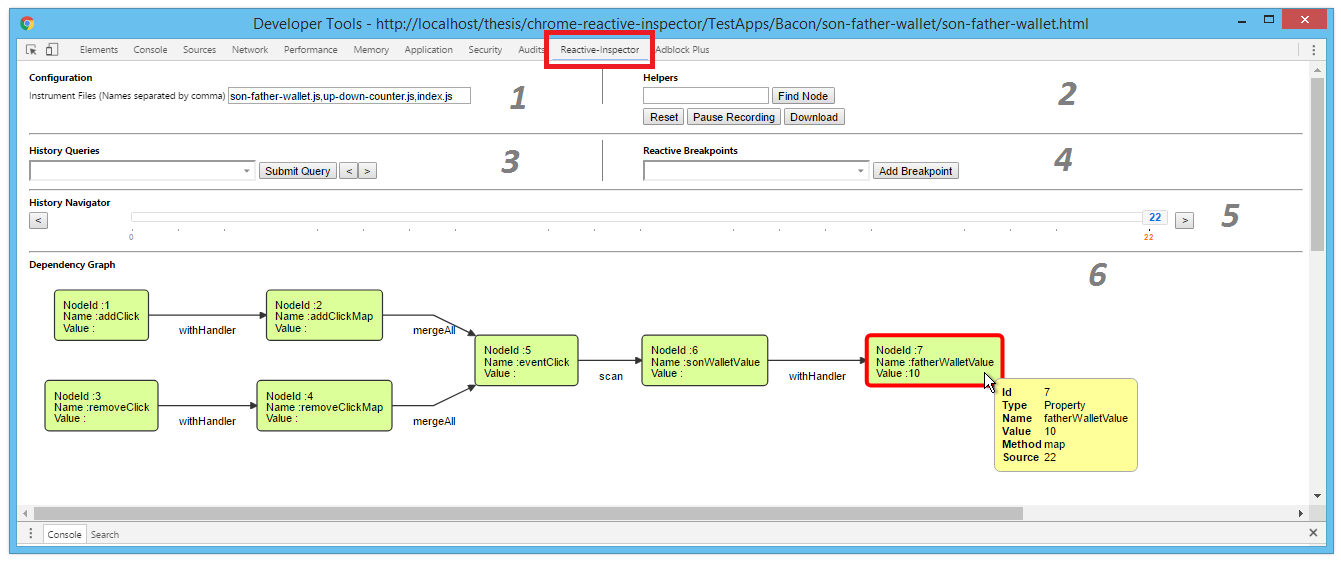
\includegraphics[scale=0.5,trim=0 0 0 0]{gfx/CRI-GUI.png}
	\caption{CRI - Graphical User Interface}
	\label{fig:system_implementation_detail}
\end{figure}

The third part of the view is to query the dependency graph, where
the developer can enter the queries explained in section~\ref{sec:The Query Language}. If a valid query is entered and the \textbf{Submit Query} button is pressed, the visualisation will jump to the first point in time at which the entered query matches. In the case of more results to a query, one can use navigation buttons available in this part to traverse through query results. The fourth part of the view is to set reactive breakpoints using the same query language that is used to search through the history of the dependency graph. 

The fifth part of the view is to navigate through the history of dependency graph with the help of a slider. One can navigate step-by-step with the help of buttons available on the left and right side of the slider. One can also use the mouse by dragging and dropping the pointer of the slider to any step. Every change to slider will result in changes to the dependency graph to a specific state. 

Last but not the least, the sixth part of the view contains the dependency graph. One can use the mouse to zoom in or out the current visualisation. Additional information to the nodes will be presented as a tooltip, if the developer hovers with the mouse over a specific node.The current node is highlighted with a red border around node box in the dependency graph.

The visualisation of the dependency graph is based on dagre-d3\footnote{\url{https://github.com/cpettitt/dagre-d3} , last accessed 25-05-2017}, which is a JavaScript library that acts as a front-end to dagre\footnote{\url{https://github.com/cpettitt/dagre} , last accessed 25-05-2017}, providing actual rendering using D3\footnote{\url{https://d3js.org/}, last accessed 25-05-2017}.